\documentclass[10pt,landscape]{article}
\usepackage[utf8]{inputenc}
\usepackage[ngerman]{babel}
\usepackage[table]{xcolor}
%\usepackage{tikz}
%\usetikzlibrary{shapes,positioning,arrows,fit,calc,graphs,graphs.standard}
\usepackage[nosf]{kpfonts}
\usepackage[t1]{sourcesanspro}
%\usepackage[lf]{MyriadPro}
%\usepackage[lf,minionint]{MinionPro}
\usepackage{multicol}
\usepackage{wrapfig}
\usepackage[absolute,overlay]{textpos}
\usepackage[top=4mm,bottom=10mm,left=4mm,right=4mm]{geometry}
\usepackage[shortlabels]{enumitem}
\usepackage[framemethod=tikz]{mdframed}
\usepackage{microtype}
\usepackage{amsmath}
\usepackage{amsfonts}
\usepackage{mathtools}
\usepackage{dirtytalk}
\usepackage{listings}
\usepackage{longtable}
\usepackage{supertabular}
\usepackage{hyperref}
\usepackage{comment}
\usepackage{soul}
\usepackage{menukeys}
\usepackage{applekeys}
\usepackage{adjustbox}
\usepackage{array}
%\usepackage{tabto}

\let\bar\overline
\newcommand{\Lim}[1]{\raisebox{0.5ex}{\scalebox{0.8}{$\displaystyle \lim_{#1}\;$}}}

\DeclarePairedDelimiter\abs{\lvert}{\rvert}%
%\setlist[enumerate,1]{leftmargin=5mm}
\setlist[itemize,1]{leftmargin=5mm}
\setlist{nosep}
\setuldepth{u}


\definecolor{myblue}{cmyk}{1,.72,0,.38}
\definecolor{mygrey}{RGB}{54,71,76}
\definecolor{vestablue}{HTML}{2B3F48}
\definecolor{pastelred}{HTML}{fbb4ae}
\definecolor{pastelblue}{HTML}{b3cde3}
\definecolor{pastelgreen}{HTML}{ccebc5}
\definecolor{pastelpurple}{HTML}{decbe4}
\definecolor{pastelorange}{HTML}{fed9a6}
\definecolor{pastelyellow}{HTML}{ffffcc}
\definecolor{pastelbrown}{HTML}{e5d8bd}
\definecolor{pastelpink}{HTML}{fddaec}
\definecolor{pastelgrey}{HTML}{f2f2f2}
\definecolor{forestgreen}{HTML}{228B22}

\def\firstcircle{(0,0) circle (1.5cm)}
\def\secondcircle{(0:2cm) circle (1.5cm)}

\colorlet{circle edge}{myblue}
\colorlet{circle area}{myblue!5}

\tikzset{filled/.style={fill=circle area, draw=circle edge, thick},
    outline/.style={draw=circle edge, thick}}

\pgfdeclarelayer{background}
\pgfsetlayers{background,main}

\everymath\expandafter{\the\everymath \color{myblue}}
\everydisplay\expandafter{\the\everydisplay \color{myblue}}

\renewcommand{\baselinestretch}{.8}
\pagestyle{empty}

%\newcommand*\rot{\rotatebox{90}}
\newcolumntype{R}[2]{%
    >{\adjustbox{angle=#1,lap=\width-(#2)}\bgroup}%
    l%
    <{\egroup}%
}
\newcommand*\rot{\multicolumn{1}{R{90}{0mm}}}% no optional argument here, please!


\global\mdfdefinestyle{header}{%
linecolor=gray,linewidth=1pt,%
leftmargin=1mm,rightmargin=2mm,
}

\newcommand{\header}{
\begin{mdframed}[]
\footnotesize
\sffamily
\Large{\textbf{Observable}} \footnotesize Cheatsheet\\
~page~\thepage~of~2
\end{mdframed}
}

\newenvironment{cde}
    {
    \fboxsep1pt
    \colorbox{gray!30}}
    {
    }

\newenvironment{cdeh}[1]
    {
    \fboxsep0pt
    \colorbox{pastelgrey}\href{#1}{}
    {}
    }

    
%\newenvironment{code}
%    {\begin{minipage}{4cm}}
 %   {\end{minipage}}
    
 
\newcommand{\entry}[3]{%%%
    \begin{minipage}{{#1}}%%
        \cde{#2}%%%
    \end{minipage}%%%
    \# #3
}%%%

\newcommand{\entryh}[4]{%%%
    \begin{minipage}{{#1}}%%
        \href{#4}{\cde{#2}}%%%
    \end{minipage}%%%
    \# #3
}%%%


\newcommand{\subsec}[2]{
\subsection*{
\begin{minipage}{32mm}
{#1}
\end{minipage}
[\texttt{#2}]}
}

%%%%%%%%%%%%%%%%%%%%%%%%%%%%%%%%%%%%%%%%%%%%%%
%% API command for columns of modules       %%
%%%%%%%%%%%%%%%%%%%%%%%%%%%%%%%%%%%%%%%%%%%%%%
\makeatletter 
\newcommand{\api}{%
  \begin{footnotesize}
  \@apii
}
\newcommand\@apii{\@ifnextchar\stopapi{\@apiend}{\@apiii}}

\newcommand\@apiii[2]{%
  \@apiiii{#1}{#2}\hfill
  \@apii % restart the recursion
}
\newcommand\@apiiii[2]{%
  \begin{minipage}[t]{{#1}}
  {#2}
  \end{minipage}}
\newcommand\@apiend[1]{% The argument is \stopapi
  \end{footnotesize}
}
\makeatother
%%%%%%%%%%%%%%%%%%%%%%%%%%%%%%%%%%%%%%%%%%%%%%%
%%%%%%%%%%%%%%%%%%%%%%%%%%%%%%%%%%%%%%%%%%%%%%%

\lstset{%
  basicstyle=\small\ttfamily,
  %breaklines=false,
  backgroundcolor = \color{pastelgrey},
  language=[LaTeX]{TeX}
}

\makeatletter
\renewcommand{\section}{\@startsection{section}{1}{0mm}%
                                {1.6ex}%
                                {.2ex}%x
                                {\color{myblue}\sffamily\Large\bfseries}}
\renewcommand{\subsection}{\@startsection{subsection}{1}{0mm}%
                                {.6ex}%
                                {.2ex}%x
                                {\sffamily\bfseries}}


\makeatother
\setlength{\parindent}{0pt}

\begin{document}
\small
\begin{multicols*}{4}
\header
\section{\href{https://github.com/observablehq/stdlib}{Standard Library}}


%%%%%%%%%%%%%%%%%%%%%%%%%%%%%%
\subsec{\href{https://github.com/observablehq/stdlib\#dom}{Dom}}{observable}

\api
{1.5cm}{
canvas\\
input \\
text
}
{1.5cm}{
context2d \\
range \\
uid
}
{1.5cm}{
download \\
select \\
}
{1.5cm}{
element \\
svg \\
}\stopapi


%%%%%%%%%%%%%%%%%%%%%%%%%%%%%%
\subsec{\href{https://github.com/observablehq/stdlib\#files}{Files}}{observable}

\api%
{2cm}{
buffer
}%
{2cm}{
text
}%
{2cm}{url
}\stopapi


%%%%%%%%%%%%%%%%%%%%%%%%%%%%%%
\subsec{\href{https://github.com/observablehq/stdlib\#file-attachments}{FileAttachments}}{\textit{attachment}}
\entry{45mm}{achmt = FileAttachment(\textquotedbl file\textquotedbl)}{construct}\\
\api%
{1.5cm}{
url\\
tsv\\
blob
}%
{1.5cm}{
text\\
image
}%
{1.5cm}{
json\\
arrayBuffer
}{1.5cm}{
csv\\
stream
}\stopapi


%%%%%%%%%%%%%%%%%%%%%%%%%%%%%%
\subsec{\href{https://observablehq.com/@observablehq/introduction-to-promises}{Promises}}{observable}
\api%
{2cm}{
delay
}%
{2cm}{
tick
}%
{2cm}{
when
}\stopapi


%%%%%%%%%%%%%%%%%%%%%%%%%%%%%%
\subsec{\href{https://github.com/observablehq/stdlib\#generators}{Generators}}{observable}
\api%
{2cm}{
disposable\\
map\\
range
}%
{2cm}{
filter\\
observe\\
valueAt
}%
{2cm}{
input\\
queue\\
worker
}\stopapi


%%%%%%%%%%%%%%%%%%%%%%%%%%%%%%
\subsec{\href{https://github.com/observablehq/stdlib\#require}{Require}}{\textit{require}}
\entry{37mm}{req = require(\textquotedbl d3-array\textquotedbl)}{from \href{https://jsdelivr.com/}{JSDelivr}}\\
\api%
{3cm}{
resolve
}%
{3cm}{
alias
}\stopapi


%%%%%%%%%%%%%%%%%%%%%%%%%%%%%%
\subsec{\href{https://github.com/observablehq/stdlib\#html}{Literals}}{observable}
\textit{The following are top-level objects. See sections on markdown and literals.}\\
\api%
{1.5cm}{
\href{https://github.com/observablehq/stdlib\#md}{md}
}%
{1.5cm}{
\href{https://github.com/observablehq/stdlib\#html}{html}
}%
{1.5cm}{
\href{https://github.com/observablehq/stdlib\#tex}{tex}
}
{1.5cm}{
\href{https://github.com/observablehq/stdlib\#dot}{dot}
}\stopapi


%%%%%%%%%%%%%%%%%%%%%%%%%%%%%%
\subsec{Reactive Variables}{observable}
\textit{These are top level objects that observe and react to changes on the notebook and server.}\\
\api%
{2cm}{
invalidation
}%
{2cm}{
now
}%
{2cm}{
width
}\stopapi


\section{\href{https://observablehq.com/@observablehq/introduction-to-data}{Data}}


%%%%%%%%%%%%%%%%%%%%%%%%%%%%%%
\subsection*{Inline}
\textit{For small datasets:}\\
\entry{44mm}{primes = [2,3,5,7,11]}{manual entry}\\
\entry{44mm}{csv = d3.csvParse(\textasciigrave rawPaste\textasciigrave)}{copy-paste}\\


%%%%%%%%%%%%%%%%%%%%%%%%%%%%%%
\subsection*{\href{https://observablehq.com/@observablehq/file-attachments}{Attachments}}

\textit{Attach a file in the UI and then:}\\
\entry{37mm}{a = FileAttachment(\textquotedbl file\textquotedbl)}{\ul{a}ttachment object}\\
\entry{37mm}{d = await a.json();}{promised \ul{d}ata}\\
\entry{37mm}{t = d3.hierarchy(d)}{in-mem \ul{t}ree}\\

\textit{In lieu of d3, }\cde{FileAttachment}\textit{ has its own csv, json, and text parsers that implicitly {\rm\bf await}:}\\
%\entry{43mm}{j = FileAttachment(\textquotedbl x.json\textquotedbl)}{json}\\
%\entry{43mm}{t = FileAttachment(\textquotedbl x.txt\textquotedbl)}{text}\\
\cde{c = FileAttachment(\textquotedbl x.csv\textquotedbl).csv()}\\
%\entry{43mm}{i = FileAttachment(\textquotedbl x.png\textquotedbl)}{image}\\

\textit{Alternatively, \href{https://observablehq.com/@mbostock/reading-local-files}{upload directly from local f.s.}:}\\
\cde{viewof file = html\textasciigrave<input type=file>\textasciigrave}\\
{\footnotesize \cde{html\textasciigrave <img src=\textquotedbl\$\{URL.createObjectURL(file)\}\textquotedbl>\textasciigrave}}\\


%%%%%%%%%%%%%%%%%%%%%%%%%%%%%%
\subsection*{\href{https://observablehq.com/@observablehq/databases}{Databases}}
\textit{Observable is meant to share notebooks and data. It is also great for prototyping. Using the runtime, you may even use it to construct full web-apps. However, notebooks themselves are not meant to serve full applications. Hence, \href{https://observablehq.com/@observablehq/databases}{UI-created db connections} are only allowed for private notebooks.}\\
\cde{npm install -g @observablehq/database-proxy}\\
\entry{45mm}{\dots}{\href{https://observablehq.com/@observablehq/self-hosted-database-proxies}{run locally}}\\

%%%%%%%%%%%%%%%%%%%%%%%%%%%%%%
\subsection*{\href{https://observablehq.com/@observablehq/secrets}{Secrets}}
\textit{Use the UI to create a secret (a la Github). Then:}\\
\entry{30mm}{Secret(\textasciigrave MY\_KEY\textasciigrave)}{expose it, or embed:}\\
\cde{dat = d3Fetch.json(url + \{\textasciigrave MY\_KEY\textasciigrave\}}\\
%\cde{\phantom{xxx}\textasciigrave https://api.nasa.gov/insight\_weather/}\\
%\cde{\phantom{xxx}?api\_key=\$\{Secret(\textasciigrave MY\_KEY\textasciigrave)\}}\\
%\cde{\phantom{xxx}\&feedtype=json\&ver=1.0\textasciigrave)}\\


%%%%%%%%%%%%%%%%%%%%%%%%%%%%%%
\subsection*{\href{https://github.com/observablehq/stdlib}{Files}}
\textit{Use this API to \href{https://observablehq.com/@mbostock/reading-local-files}{retrieve from local filesystem}.}\\
\cde{viewof myText = html\textasciigrave<input type=file>\textasciigrave}\\
\entry{35mm}{Files.text(myText)}{invoke the API}\\

\section{\href{https://observablehq.com/@observablehq/inputs}{Inputs}}

%%%%%%%%%%%%%%%%%%%%%%%%%%%%%
\subsection*{General Use}
\entry{45mm}{import \{Checkbox\} from \dots}{from \href{https://observablehq.com/@observablehq/inputs}{here}}\\
\entry{45mm}{data = [\dots]; options = \{\dots\};}{setup}\\
\entry{52mm}{viewof cb = Checkbox(data, options)}{create}\\
\entry{45mm}{html\textasciigrave checked: }{reference}\\
\cde{\phantom{xxxx}\$\{cb.map(c => html\textasciigrave \$\{c\}\textasciigrave)\}\textasciigrave}\\

\textit{Most canonical inputs have the 2 arguments above, where }\cde{data}\textit{ is an array, and }\cde{options}\textit{ is an object-literal, as described below.}\\

%%%%%%%%%%%%%%%%%%%%%%%%%%%%%
\subsection*{Options}
\textit{Most inputs allow arbitrarily-formatted }\cde{data}\textit{ but then require using non-trivial }\cde{keysof}, \cde{valuesof}\textit{ closures for data extraction. Other options are mostly cosmetic.}\\

\addtolength{\tabcolsep}{-3pt}    
{\footnotesize
\rowcolors{0}{gray!20}{white}
\begin{tabular}{@{} rp{3mm}p{3mm}p{3mm}p{3mm}p{3mm}p{3mm}p{3mm}p{3mm}p{3mm}p{3mm} @{}}
                & \rot{Button}  & \rot{Chckbx}  & \rot{Toggle}  & \rot{Radio}   & \rot{Range}   & \rot{Search}  & \rot{Text}    & \rot{Textar.} & \rot{Select}  & \rot{Table}   \\
    Label       & \checkmark    & \checkmark    & \checkmark    & \checkmark    & \checkmark    & \checkmark    & \checkmark    & \checkmark    & \checkmark    &               \\
    Value       & \checkmark    & \checkmark    & \checkmark    &               & \checkmark    &               & \checkmark    & \checkmark    & \checkmark    & \checkmark    \\
    Width       & \checkmark    &               &               &               & \checkmark    & \checkmark    & \checkmark    & \checkmark    & \checkmark    & \checkmark    \\
    Disabl'd    & \checkmark    & \checkmark    & \checkmark    & \checkmark    & \checkmark    & \checkmark    & \checkmark    & \checkmark    & \checkmark    &               \\
    Sort        &               & \checkmark    &               & \checkmark    &               &               &               &               & \checkmark    & \checkmark    \\
    Unique      &               & \checkmark    &               & \checkmark    &               &               &               &               & \checkmark    &               \\
    Locale      &               & \checkmark    &               & \checkmark    &               & \checkmark    &               &               & \checkmark    &               \\
    Format      &               & \checkmark    &               & \checkmark    & \checkmark    & \checkmark    &               &               & \checkmark    & \checkmark    \\
    Keyof       &               & \checkmark    &               & \checkmark    &               &               &               &               & \checkmark    &               \\
    Valueof     &               & \checkmark    &               & \checkmark    &               &               &               &               & \checkmark    &               \\
    Plachldr    &               &               &               &               & \checkmark    & \checkmark    & \checkmark    & \checkmark    &               &               \\
    Columns     &               &               &               &               &               & \checkmark    &               &               &               & \checkmark    \\
    Sp'lch'k    &               &               &               &               &               & \checkmark    & \checkmark    & \checkmark    &               &               \\
    Requ'd      &               &               &               &               &               & \checkmark    & \checkmark    & \checkmark    &               & \checkmark    \\
    Rows        &               &               &               &               &               &               &               & \checkmark    &               & \checkmark    \\
    Datalst     &               &               &               &               &               & \checkmark    & \checkmark    &               &               &               \\
    Multip.     &               &               &               &               &               &               &               &               & \checkmark    & \checkmark    \\
    Reado'ly    &               &               &               &               &               &               & \checkmark    & \checkmark    &               &               \\
    Minlen.     &               &               &               &               &               &               & \checkmark    & \checkmark    &               &               \\
    Maxlen.     &               &               &               &               &               &               & \checkmark    & \checkmark    &               &               \\
    Validate    &               &               &               &               &               &               & \checkmark    & \checkmark    &               &               \\
    Submit      &               &               &               &               &               &               & \checkmark    & \checkmark    &               &               \\
\end{tabular}}
\addtolength{\tabcolsep}{3pt}
\\
\textit{The following are exclusive to one input type:}
\begin{itemize}
    \item button \tabto{15mm} required, reduce
    \item toggle \tabto{15mm} values
    \item range \tabto{15mm} step, transform, invert
    \item select \tabto{15mm} size
    \item text \tabto{15mm} type, pattern
    \item search \tabto{15mm} query, filter
    \item table \tabto{15mm} reverse, align, maxwidth, height, maxHeight, layout
\end{itemize}


%%%%%%%%%%%%%%%%%%%%%%%%%%%%%
\subsection*{Idiosyncratic / User-defined Inputs}



\begin{minipage}{3cm}
\begin{itemize}
    \item \href{https://observablehq.com/@mootari/2d-slider}{2D Slider}
    \item \href{https://observablehq.com/@rreusser/binary-input}{Binary Input}
    \item \href{https://observablehq.com/@yurivish/ternary-slider}{Ternary Slider}
    \item \href{https://observablehq.com/@rreusser/fine-range}{Fine-range Slider}
    \item \href{https://observablehq.com/@mbostock/form-input}{Form Input}
    \item \href{https://observablehq.com/@mootari/range-slider}{Range Slider}
\end{itemize}
\end{minipage}\begin{minipage}{3cm}
\begin{itemize}
    \item \href{https://observablehq.com/@mbostock/scrubber}{Scrubber}
    \item \href{https://observablehq.com/@oscar6echo/player}{Player}
    \item \href{https://observablehq.com/@bumbeishvili/input-groups}{Inputs in a Grid}
    \item \href{https://observablehq.com/@mbostock/copier}{Copier}
    \item \href{https://observablehq.com/@awhitty/fips-county-code-brush}{US Counties}
    \item \href{https://observablehq.com/@bobkerns/elements-input}{Periodic Table}
\end{itemize}
\end{minipage}
\section{Imports \& Exports}


%%%%%%%%%%%%%%%%%%%%%%%%%%%%%%
\subsection*{Cell Imports}
\textit{Successively: static import; multiple cells; with dependency injection; aliasing; non-public.}\\
\cde{import \{chart\} from '@mbostock/phases-moon'}\\
\cde{import \{chart, viewof year\} from \dots}
\cde{import \{chart\} with \{mydata as data\} from \dots}\\
\cde{import \{chart as barchar\} \dots}\\


\textit{Note: Imported cells evaluate dependencies without binding them to the local notebook. Bindings are live ($\Delta$ with underlying dependencies), but lazily evaluated.}
%\begin{comment}\begin{wrapfigure}[2]{r}{10mm}
%\vspace{-4mm}
%\resizebox{10mm}{!}{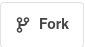
\includegraphics[]{img/fork.jpg}}
%\end{wrapfigure}\end{comment}
\textit{Since you can only import \textbf{named} cells, consider ``forking'' a notebook instead.}\\


%%%%%%%%%%%%%%%%%%%%%%%%%%%%%%
\subsection*{\href{https://observablehq.com/@observablehq/introduction-to-require}{Require}}
\textit{Used for plain JavaScript library imports.}\\
\entry{43mm}{mmnt = require("moment")}{\href{https://momentjs.com/}{moment} lib}\\
\entry{43mm}{mmnt = require("moment@2")}{vers. 2}\\
\entry{43mm}{ab = require("a", "b")}{multiple $\to$ 1}\\

\textit{Libs fetch from \href{https://www.npmjs.com/}{npm} by default. Override like:}\\
\entry{49mm}{d3 = require("my.server/d3.js")}{www loc}\\
\entry{49mm}{d3 = require("localhost/d3.js")}{local}\\

\textit{As an alternative, consider \href{https://exploringjs.com/es6/ch\_modules.html}{ES6-native imports}:}\\
\cde{d3\_esm = import(\textquotedbl https://some.cdn/d3@6\textquotedbl)}\\


%%%%%%%%%%%%%%%%%%%%%%%%%%%%%%
\subsection*{Sharing}
\textit{Notebooks default to ``private'' access but can also be ``shared'' (exposing an obfuscated url) or ``published,'' all as available in the UI. Alternatively, click to left of a cell to download its contents to png or json, etc.}


%%%%%%%%%%%%%%%%%%%%%%%%%%%%%%
\subsection*{\href{https://observablehq.com/@observablehq/introduction-to-embedding?collection=@observablehq/embedding-notebooks}{Embedding}}
\textit{To the left of a cell, select ``embed'' to generate copy-pasteable html }\texttt{IFrame}\textit{ code (which will, in turn, include the observable runtime). \href{https://observablehq.com/@jashkenas/handy-embed-code-generator}{Here} is a tool that generates an IFrame for multiple cells. Alternatively, download a zip archive of project contents by clicking ``download code.'' The generated archive is described \href{https://www.tophtucker.com/observable-docco/index.js.html}{here}. Even better, just install it via npm using the url in the download code menu option:}\\
\cde{unix-shell\$ @observablehq/runtime}\\
\cde{unix-shell\$ npm install \textquotedbl <url>\textquotedbl}


%%%%%%%%%%%%%%%%%%%%%%%%%%%%%%
\subsection*{\href{https://observablehq.com/@observablehq/downloading-and-embedding-notebooks}{Observable Runtime}}
{\it A {\rm \href{https://github.com/observablehq/runtime}{\cde{Runtime}}} instance can spawn a {\rm\tt \cde{module}}, which, when passed an {\rm \href{https://github.com/observablehq/runtime#modules}{\cde{observer}}}, spawns a {\rm \href{https://github.com/observablehq/runtime#variables}{\cde{variable}}}, which is a piece of state in a reactive program. The standard observer is {\rm\tt \href{https://github.com/observablehq/inspector}{\cde{Inspector}}}, which renders the current value of the given variable to its associated DOM element.}

\cde{<html><body><script type=\textquotedbl module\textquotedbl>}\\
\cde{import \{Runtime, Inspector\} from \dots}\\
\cde{import define from \textquotedbl https://\dots\textquotedbl;}\\
\cde{const runtime = new Runtime();}\\
\cde{const main = runtime.module(define, }\\
\cde{ \phantom{xxx} name => \{ if (name === \textquotedbl hello\textquotedbl) \{ }\\
\cde{ \phantom{xxxxxx} return new Inspector(document.body);}\\
\cde{ \phantom{xxx}  \} }\\
\cde{\});}\\
\cde{</script>}\\
\section{Markdown}

%%%%%%%%%%%%%%%%%%%%%%%%%%%%%%%%%%
\subsection*{Headers}

\entry{35mm}{\# \, Title}{H1 header}\\
\entry{35mm}{\#\#\, Title}{H2 header}\\
\entry{35mm}{\#\#\#\, Title}{H3 header}\\

%%%%%%%%%%%%%%%%%%%%%%%%%%%%%%%%%%
\subsection*{Emphasis}

\entry{35mm}{**text**}{bold \textbf{text}}\\
\entry{35mm}{\_ text\_}{italicized \textit{text}  }\\
\entry{35mm}{\textasciitilde\textasciitilde text\textasciitilde\textasciitilde}{striken-thru \st{text}}\\
\entry{35mm}{> text}{quoted text}\\

%%%%%%%%%%%%%%%%%%%%%%%%%%%%%%%%%%%
\subsection*{Hyperlinks, Images, \& Videos}
\cde{[http://google.com](click here!)}\\
\cde{![http://clip.art](pic's subtitle)}\\

\textit{Embed youtube video:}\\
\cde{[![description]}\\
\cde{(http://img.youtube.com/vi/myvidid/0.jpg)]}\\
\cde{(http://www.youtube.com/watch?v=myvidid)}\\


%%%%%%%%%%%%%%%%%%%%%%%%%%%%%%%
\subsection*{Lists}


\begin{tabular}{l l}
    \ul{Unordered} & \ul{Ordered} \\
    \cde{* item1} & \cde{1. item1} \\ 
    \cde{* item2} & \cde{1. item2} \\
    \cde{* item3} & \cde{1. item3} \\
\end{tabular}

\textit{Mixed, Nested lists:}\\
\cde{1. First major item}\\
\cde{\phantom{xx} * 1st sub-item}\\
\entry{35mm}{\phantom{xx} * 2nd sub-item}{whitespace matters!}\\
\cde{1. Second major item}\\

%%%%%%%%%%%%%%%%%%%%%%%%%%%%%%%%
\subsection*{Code}

\entry{35mm}{normal \textasciigrave code()\textasciigrave text }{inline}\\
\entry{35mm}{\textasciigrave\textasciigrave\textasciigrave}{start \dots}\\
\entry{35mm}{myFunction()\{\}}{code block}\\
\entry{35mm}{\textasciigrave\textasciigrave\textasciigrave}{\dots end}\\[1mm]
\textit{In observable, backticks must be escaped (see below), so really, things look more like:}\\ 
\begin{tabular}{l l}
    \ul{template literal} & \ul{tagged TL}\\
    \cde{\textbackslash \textasciigrave\textbackslash \textasciigrave\textbackslash\textasciigrave} & \cde{\textbackslash \textasciigrave\textbackslash \textasciigrave\textbackslash\textasciigrave html} \\
    \cde{myFunction()\{\}} & \cde{<i>ital</i>} \\
    \cde{\textbackslash\textasciigrave\textbackslash\textasciigrave\textbackslash\textasciigrave} & \cde{\textbackslash \textasciigrave\textbackslash \textasciigrave\textbackslash\textasciigrave} \\
\end{tabular}

%%%%%%%%%%%%%%%%%%%%%%%%%%%%
\subsection*{Escaping}
\textit{The following characters must be escaped: \cde{*}, and \cde{>}. Within observable, additionally escape \cde{\textasciigrave}.}\\

%%%%%%%%%%%%%%%%%%%%%%%%%%%%
\subsection*{Tables}
\textit{For all but the simplest tables, embed html, but for simple tables, use raw markdown syntax:}\\
\entry{40mm}{| head1 | head2 | head3 |}{headers}\\
\entry{40mm}{|-------|-------|-------|}{horizontal rule}\\
\entry{40mm}{| val   | val   | val   |}{rows}\\


%%%%%%%%%%%%%%%%%%%%%%%%%%%%
\subsection*{Checklists}
\entry{30mm}{- [ ] Mercury}{unchecked}\\
\entry{30mm}{- [x] Venus}{checked}\\
\entry{30mm}{- [x] Earth}{note: '-' for list}\\
\entry{30mm}{- [ ] Mars}{space $\leftrightarrow$ empty}\\

%%%%%%%%%%%%%%%%%%%%%%%%%%%%%%%%%%%%%%%%%
\subsection*{\href{https://observablehq.com/@mbostock/html-in-markdown}{HTML}}
\textit{Most html can be embedded successfully. Some idioms are below, the first of which is used to add dynamic html text highlighting:}\\
\cde{<span \$\{spanStyle('link')\}>*Link*</span> }\\
\entry{45mm}{<span>\&\# 10004<\textbackslash span>}{unicode char}\\[1mm]
\entry{35mm}{<dl>}{begin definition list}\\
\entry{35mm}{<dt></dt>}{definition header}\\
\entry{35mm}{<dd></dd>}{definition}\\
\entry{35mm}{</dl>}{end }\\[1mm]
\entry{48mm}{<figcaption>text</figcaption>}{nice captn}\\
\entry{48mm}{<figure style='max-width:50px'>}{nice image}\\
\entry{48mm}{<img src='https://pic.location'>}{}\\
\entry{48mm}{</figure>}{end}\\


\section{Literals}

\textit{No matter the language below, observable always requires ``tagging'' the ``\href{https://exploringjs.com/es6/ch_template-literals.html\#\_tagged-template-literals}{template literal},'' by prefixing the target language prior to the template-demarcating graves (}\cde{\textasciigrave}\textit{).}

%%%%%%%%%%%%%%%%%%%%%%%%%%%%%%
\subsection*{\href{}{Markdown}}
\textit{(See separate section on md.)}\\
\cde{md\textasciigrave \# Page Title\textasciigrave}\\


%%%%%%%%%%%%%%%%%%%%%%%%%%%%%%
\subsection*{\href{https://observablehq.com/@observablehq/introduction-to-html?collection=@observablehq/notebook-fundamentals}{HTML}}
\cde{html\textasciigrave <p>I am a <i>par</i> element!</p>\textasciigrave}\\
\entry{50mm}{html\textasciigrave<style> }{this css}\\
\entry{50mm}{\phantom{xx}.highlight \{background: yellow;\}}{applies}\\
\entry{50mm}{</style>\textasciigrave}{globally}\\

%%%%%%%%%%%%%%%%%%%%%%%%%%%%%%
\subsection*{\href{https://observablehq.com/@observablehq/htl}{SVG}}
\cde{svg\textasciigrave<svg width=60 height=60>}\\
\cde{\phantom{xxx}\$\{svg.fragment\textasciigrave }\\
\cde{\phantom{xxxxx}<circle cx=30 cy=30 r=30></circle>\textasciigrave}\\
\cde{</svg>\textasciigrave}\\


%%%%%%%%%%%%%%%%%%%%%%%%%%%%%%
\subsection*{\href{https://observablehq.com/@observablehq/graphviz}{GraphViz / DOT}}
\cde{dot\textasciigrave digraph \{ a -> b; \}\textasciigrave}\\

%%%%%%%%%%%%%%%%%%%%%%%%%%%%%%
\subsection*{\TeX}
\entry{35mm}{tex\textasciigrave E = mc\textasciicircum 2\textasciigrave}{inline}\\
\entry{35mm}{tex.block\textasciigrave \dots \textasciigrave}{block-mode}\\


%%%%%%%%%%%%%%%%%%%%%%%%%%%%%%
\subsection*{Lorem Ipsem}
\textit{Really just a cell import from \href{https://observablehq.com/@jashkenas/lorem-ipsum}{here}, then:}\\
\cde{md\textasciigrave \$\{loremipsum(\{using: "Bro Ipsum"\})\}\textasciigrave}\\


%%%%%%%%%%%%%%%%%%%%%%%%%%%%%%
\subsection*{\href{https://tinyurl.com/u6y8b4pd}{Template Expansion}}
\textit{All literals are actually templates that are parsed into intermediate languages (like \TeX\ and markdown) and ultimately resolved to html. Prior to parsing, observable expands ``interpolated expressions'' (those inside \cde{\$\{\dots\}}) into their ``substituted'' string value.}\\
\cde{\textasciigrave <h1>Hello \$\{value\}</h1>\textasciigrave }


%%%%%%%%%%%%%%%%%%%%%%%%%%%%%%
\subsection*{\href{}{Nesting Literals}}
\entry{45mm}{md\textasciigrave Some tex: \$\{tex\textasciigrave \textbackslash tau\textasciigrave\}.\textasciigrave}{\TeX\ in md}\\

\textit{Deep nesting: given observable / js variable:}\\
\cde{array = [tex\textasciigrave A=1\textasciigrave, tex\textasciigrave A=2\textasciigrave]}\\
\textit{\dots nest \TeX\ inside js inside html inside js inside html inside md!}\\
\cde{md\textasciigrave A list of elements:}\\
\cde{<ul>}\\
\cde{\phantom{xxx}\$\{clone(array).map(a => html\textasciigrave<li>\$\{a\}\textasciigrave)\}}\\
\cde{</ul>\textasciigrave}\\
\section{Keyboard Shortcuts}


%%%%%%%%%%%%%%%%%%%%%%%%%%%%%%%%%%%%%%%%%%
\subsection*{Cell Editing}
\entry{25mm}{\shiftkey-\returnkey \quad \ctlkey-S}{run current cell}\\
\entry{25mm}{\optkey-\shiftkey-$\downarrow$}{focus next cell}\\
\entry{25mm}{\optkey-\shiftkey-$\uparrow$}{focus prev. cell}\\
\entry{25mm}{\optkey-\returnkey}{split cell @ cursor}\\
\entry{25mm}{\optkey-\shiftkey-\returnkey}{ibid, focusing 1st}\\
\entry{25mm}{\optkey-\returnkey}{insert cell, after}\\
\entry{25mm}{\optkey-\shiftkey-\returnkey}{insert cell, before}\\
\entry{25mm}{\optkey-\shiftkey-$\uparrow$}{move cell up}\\
\entry{25mm}{\optkey-\shiftkey-$\downarrow$}{move cell down}\\
\entry{25mm}{\optkey-\delkey}{merge cell w/ prev.}\\
\entry{25mm}{\ctlkey-\shiftkey-D}{merge cell w/ next}\\
\entry{25mm}{\ctlkey-\shiftkey-P}{[un]pin cell}\\
\entry{25mm}{\ctlkey-J}{jump to ref'd cell}\\
\entry{25mm}{\esckey}{blur current cell}\\



%%%%%%%%%%%%%%%%%%%%%%%%%%%%%%%%%%%%%%%%%%
\subsection*{Cursor}

\entry{25mm}{\ctlkey-$\leftarrow$}{previous word}\\
\entry{25mm}{\ctlkey-$\rightarrow$}{next word}\\
\entry{25mm}{\optkey-$\leftarrow$}{start line}\\
\entry{25mm}{\optkey-$\rightarrow$}{end line}\\
\entry{25mm}{\ctlkey-HOME}{to start of cell}\\
\entry{25mm}{\ctlkey-END}{to end of cell}\\
\entry{25mm}{\ctlkey-CLICK}{multiple carets}\\



%%%%%%%%%%%%%%%%%%%%%%%%%%%%%%%%%%%%%%%%%%
\subsection*{Selection}

\entry{25mm}{\shiftkey-$\leftarrow$}{extend sel. left}\\
\entry{25mm}{\shiftkey-$\rightarrow$}{extend sel. right}\\
\entry{25mm}{\shiftkey-$\uparrow$}{extend sel. up}\\
\entry{25mm}{\shiftkey-$\downarrow$}{extend sel. down}\\
\entry{25mm}{\ctlkey-\shiftkey-$\leftarrow$}{extend sel. word}\\
\entry{25mm}{\ctlkey\shiftkey-$\rightarrow$}{extend sel. word}\\
\entry{25mm}{\optkey-\shiftkey-$\leftarrow$}{to start of line}\\
\entry{25mm}{\optkey-\shiftkey-$\rightarrow$}{to end of line}\\



%%%%%%%%%%%%%%%%%%%%%%%%%%%%%%%%%%%%%%%%%%
\subsection*{Text}

\entry{25mm}{\ctlkey-BACKSPACE}{delete word before}\\
\entry{25mm}{\ctlkey-\delkey}{delete word after}\\
\entry{25mm}{\shiftkey-\tabkey}{auto-indent}\\
\entry{25mm}{\ctlkey-]}{indent once}\\
\entry{25mm}{\ctlkey-[}{de-indent once}\\
\entry{25mm}{\ctlkey-/}{toggle comment (JS-only)}\\




%%%%%%%%%%%%%%%%%%%%%%%%%%%%%%%%%%%%%%%%%%
\subsection*{Cell Navigation}

\entry{25mm}{k}{select cell above}\\
\entry{25mm}{j}{select cell below}\\
\entry{25mm}{\shiftkey-\returnkey}{run selected cells}\\
\entry{25mm}{\shiftkey-k}{expand selection up}\\
\entry{25mm}{\shiftkey-j}{expand selection down}\\
\entry{25mm}{\shiftkey-$\uparrow$}{move cells up}\\
\entry{25mm}{\shiftkey-$\downarrow$}{move cells down}\\
\entry{25mm}{o}{insert cell after}\\
\entry{25mm}{\shiftkey-o}{insert cell before}\\
\entry{25mm}{x}{toggle select cell}\\
\entry{25mm}{\shiftkey-a}{select all cells}\\
\entry{25mm}{\esckey}{deselect all cells}\\
\entry{25mm}{\returnkey}{open cell editor}\\
\entry{25mm}{d}{delete selected cells}\\
\entry{25mm}{p}{[un]pin selected cells}\\



%%%%%%%%%%%%%%%%%%%%%%%%%%%%%%%%%%%%%%%%%%
\subsection*{Other}

\entry{25mm}{\ctlkey-c}{copy selection / line}\\
\entry{25mm}{\ctlkey-x}{cut selection / line}\\
\entry{25mm}{\ctlkey-v}{paste selection / line}\\
\entry{25mm}{\ctlkey-z}{undo}\\
\entry{25mm}{\ctlkey-y}{redo}\\
\entry{25mm}{\ctlkey-f}{search text}\\
\entry{25mm}{\ctlkey-g}{find next occurrence}\\
\entry{25mm}{\ctlkey-\shiftkey-g}{previous occurrence}\\




\vfill
\,
%[25cm]

\section{Compiler}

%%%%%%%%%%%%%%%%%%%%%%%%%%%%%%%%%%%
\subsection*{Grammar}
\cde{Cell:}\\
\cde{\qquad ImportCell}\\
\cde{\qquad NamedCell}\\
\cde{\qquad Block}\\
\cde{\qquad Expression}\\
\cde{ImportCell:}\\
\cde{\qquad import NamedImports}\\
\cde{\phantom{xxxxxxxxxx}from moduleSpecifier}\\
\cde{\qquad import NamedImports }\\
\cde{\phantom{xxxxxxxxxx}with namedImports} \cde{\phantom{xxxxxxxxxx}from moduleSpecifier}\\
\cde{NamedCell:}\\
\cde{\qquad Identifier = Block}\\
\cde{\qquad Identifier = Expression}\\  
\cde{\qquad FunctionExpression}\\
\cde{\qquad ClassExpression}\\
\cde{Identifier:}\\
\cde{\qquad IdentifierName}\\
\cde{\qquad viewof IdentifierName}\\
\cde{\qquad mutable IdentifierName}\\



%%%%%%%%%%%%%%%%%%%%%%%%%%%%%%
\subsection*{Parser}
\textit{See examples \href{https://github.com/observablehq/parser}{here}, or do the following to see how parser creates a json tree or your choosing:}\\


\cde{import \{parseCell\} from "@observablehq/parser";}\\
\cde{const cell = parseCell(\textasciigrave hello = "world"\textasciigrave);}\\
\section{Misc. Techniques}
\textit{The below are cool techniques that blend much of the above in a unique, non-categorizable way:}\\
\begin{itemize}
    \item \href{https://observablehq.com/@observablehq/introducing-visual-dataflow?collection=@observablehq/introduction}{Gallery of gifs}
    \item \href{https://observablehq.com/@asg017/introduction-to-the-new-observable-prerender-cli}{CLI-based notebook rendering}
    \item \href{https://observablehq.com/@mbostock/canvas-to-gif}{GIF animations from Canvas} using \href{https://jnordberg.github.io/gif.js/}{gif.js}
\end{itemize}
\end{multicols*}
\end{document}
